\documentclass[letterpaper,landscape]{article}
\usepackage[margin=0.30in,headsep=5pt,footskip=14pt]{geometry}
\usepackage[T1]{fontenc}
\usepackage[utf8]{inputenc}
\usepackage{lmodern}
\usepackage{amsmath}
\usepackage{graphicx}
\usepackage{booktabs}
\usepackage{array}
\usepackage{tabularx}
\usepackage[table]{xcolor}
\usepackage{microtype}
\usepackage{fancyhdr}
\usepackage{hyperref}

\definecolor{navy}{HTML}{17324D}
\definecolor{pale}{HTML}{EDF4F8}
\definecolor{amber}{HTML}{8A5A00}
\definecolor{amberpale}{HTML}{FFF4D6}
\definecolor{green}{HTML}{1B6A4A}
\definecolor{gray}{HTML}{5A6570}
\hypersetup{colorlinks=true,linkcolor=navy,pdfauthor={Holstein implementation project},pdftitle={Paper II SIAM observable screening snapshot}}
\pagestyle{fancy}
\fancyhf{}
\lhead{\footnotesize\color{gray}Paper II / SIAM observable evidence}
\rhead{\footnotesize\color{gray}Built 2026-08-30}
\cfoot{\footnotesize\color{gray}\thepage}
\renewcommand{\headrulewidth}{0.3pt}
\setlength{\parindent}{0pt}
\setlength{\parskip}{1.5pt}
\newcolumntype{Y}{>{\raggedright\arraybackslash}X}
\newcommand{\statusbox}[1]{\colorbox{amberpale}{\parbox{0.975\linewidth}{\centering\strut\textcolor{amber}{\textbf{#1}}\strut}}}

\begin{document}

{\Large\bfseries\color{navy} SIAM \(N_b=4\) observable screening snapshot}\hfill
{\small\color{gray}hybridization quench, \(t\in[0,1]\)}

\statusbox{DIAGNOSTIC ONLY --- CURRENT PAIR REJECTED AS ACCURACY-CONFOUNDED; NO COST COMPARISON IS ADMISSIBLE}

\vspace{2pt}
\rowcolors{2}{pale}{white}
\begin{tabularx}{\linewidth}{@{}p{1.34in}Y@{}}
\toprule
Source aggregate & Row count: 2 locked exact-scored trajectory JSONs: \texttt{sources/siam\_avqds\_cluster9714484\_score.json} (SHA-256 \texttt{8c6125f7...35614614}) and \texttt{sources/siam\_apm\_cluster9715147\_score.json} (SHA-256 \texttt{25414cc6...19a6f2e7}). \\
Scheduler identities & AVQDS \texttt{9714484.0}, cut \(10^{-3}\); Full APM \texttt{9715147.0}, cut \(10^{-5}\), exchange policy. Each score contains 101 shared time samples on \(t=0,0.01,\ldots,1\). Evidence revision \texttt{d5590449}; run code \texttt{36c40d52}. \\
Identity audit & \textcolor{green}{\textbf{PASS\_DIAGNOSTIC\_COMPARISON\_IDENTITY}}: identical grid, seed, Hamiltonian/physics fingerprint, comparison fingerprint, observable contract, exact observable arrays, and exact-energy arrays. \\
Observable definitions & \(m_d=\langle n_{d\uparrow}-n_{d\downarrow}\rangle\), \(D_d=\langle n_{d\uparrow}n_{d\downarrow}\rangle\), \(C_j=\langle\mathbf S_d\!\cdot\!\mathbf S_j\rangle\) including transverse exchange, and Sigma-v2 \(\Sigma_r=\langle S_d^2\rangle+\sum_{j=1}^{r}C_j\), with \(\langle S_d^2\rangle=\tfrac34(N_d-2D_d)\). \\
Interpretation & Exact evolution is reporting-only and was not used by either controller. Neither trajectory passes the individual 5\% primitive-response target. Full APM fails the 15\% broad guard in the tiny-response \(C_3\) channel, so the pair is accuracy-confounded. Qiskit compilation was not performed. \\
\bottomrule
\end{tabularx}
\rowcolors{2}{}{}

\vspace{2pt}
\begin{center}
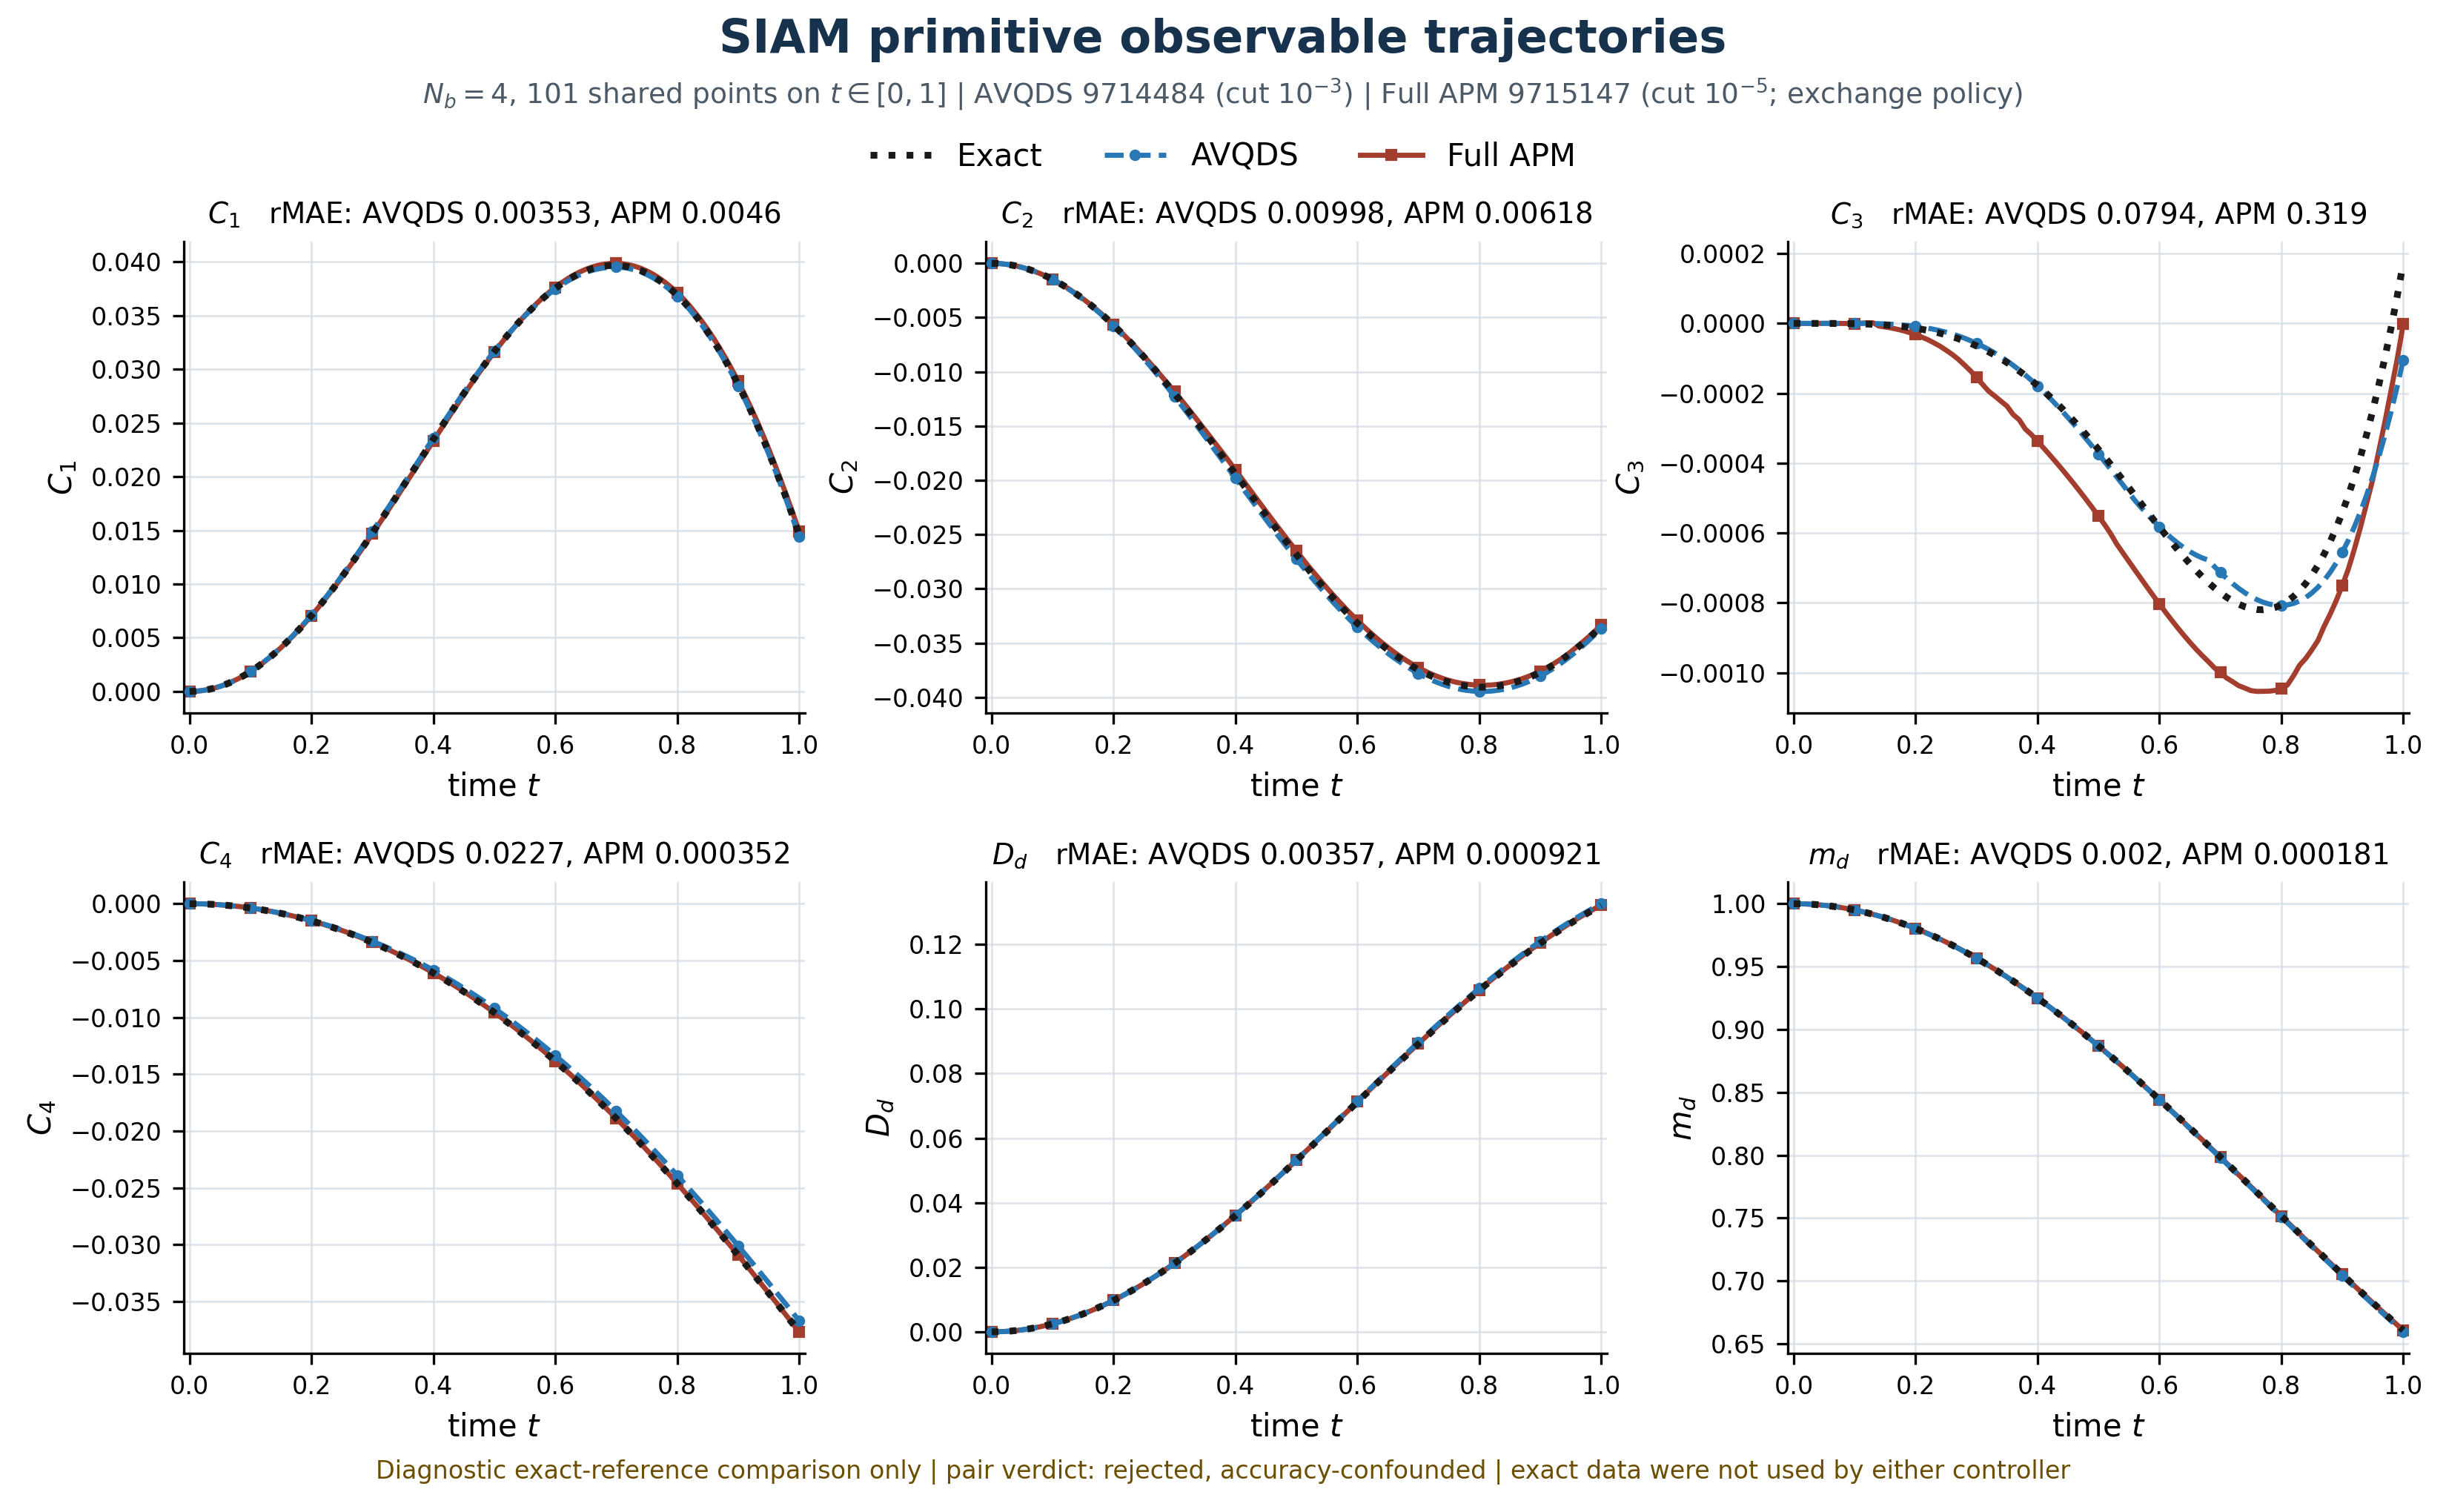
\includegraphics[width=0.84\linewidth,height=4.75in,keepaspectratio]{siam_nb4_primitive_observables.png}
\end{center}

\newpage
\begin{center}
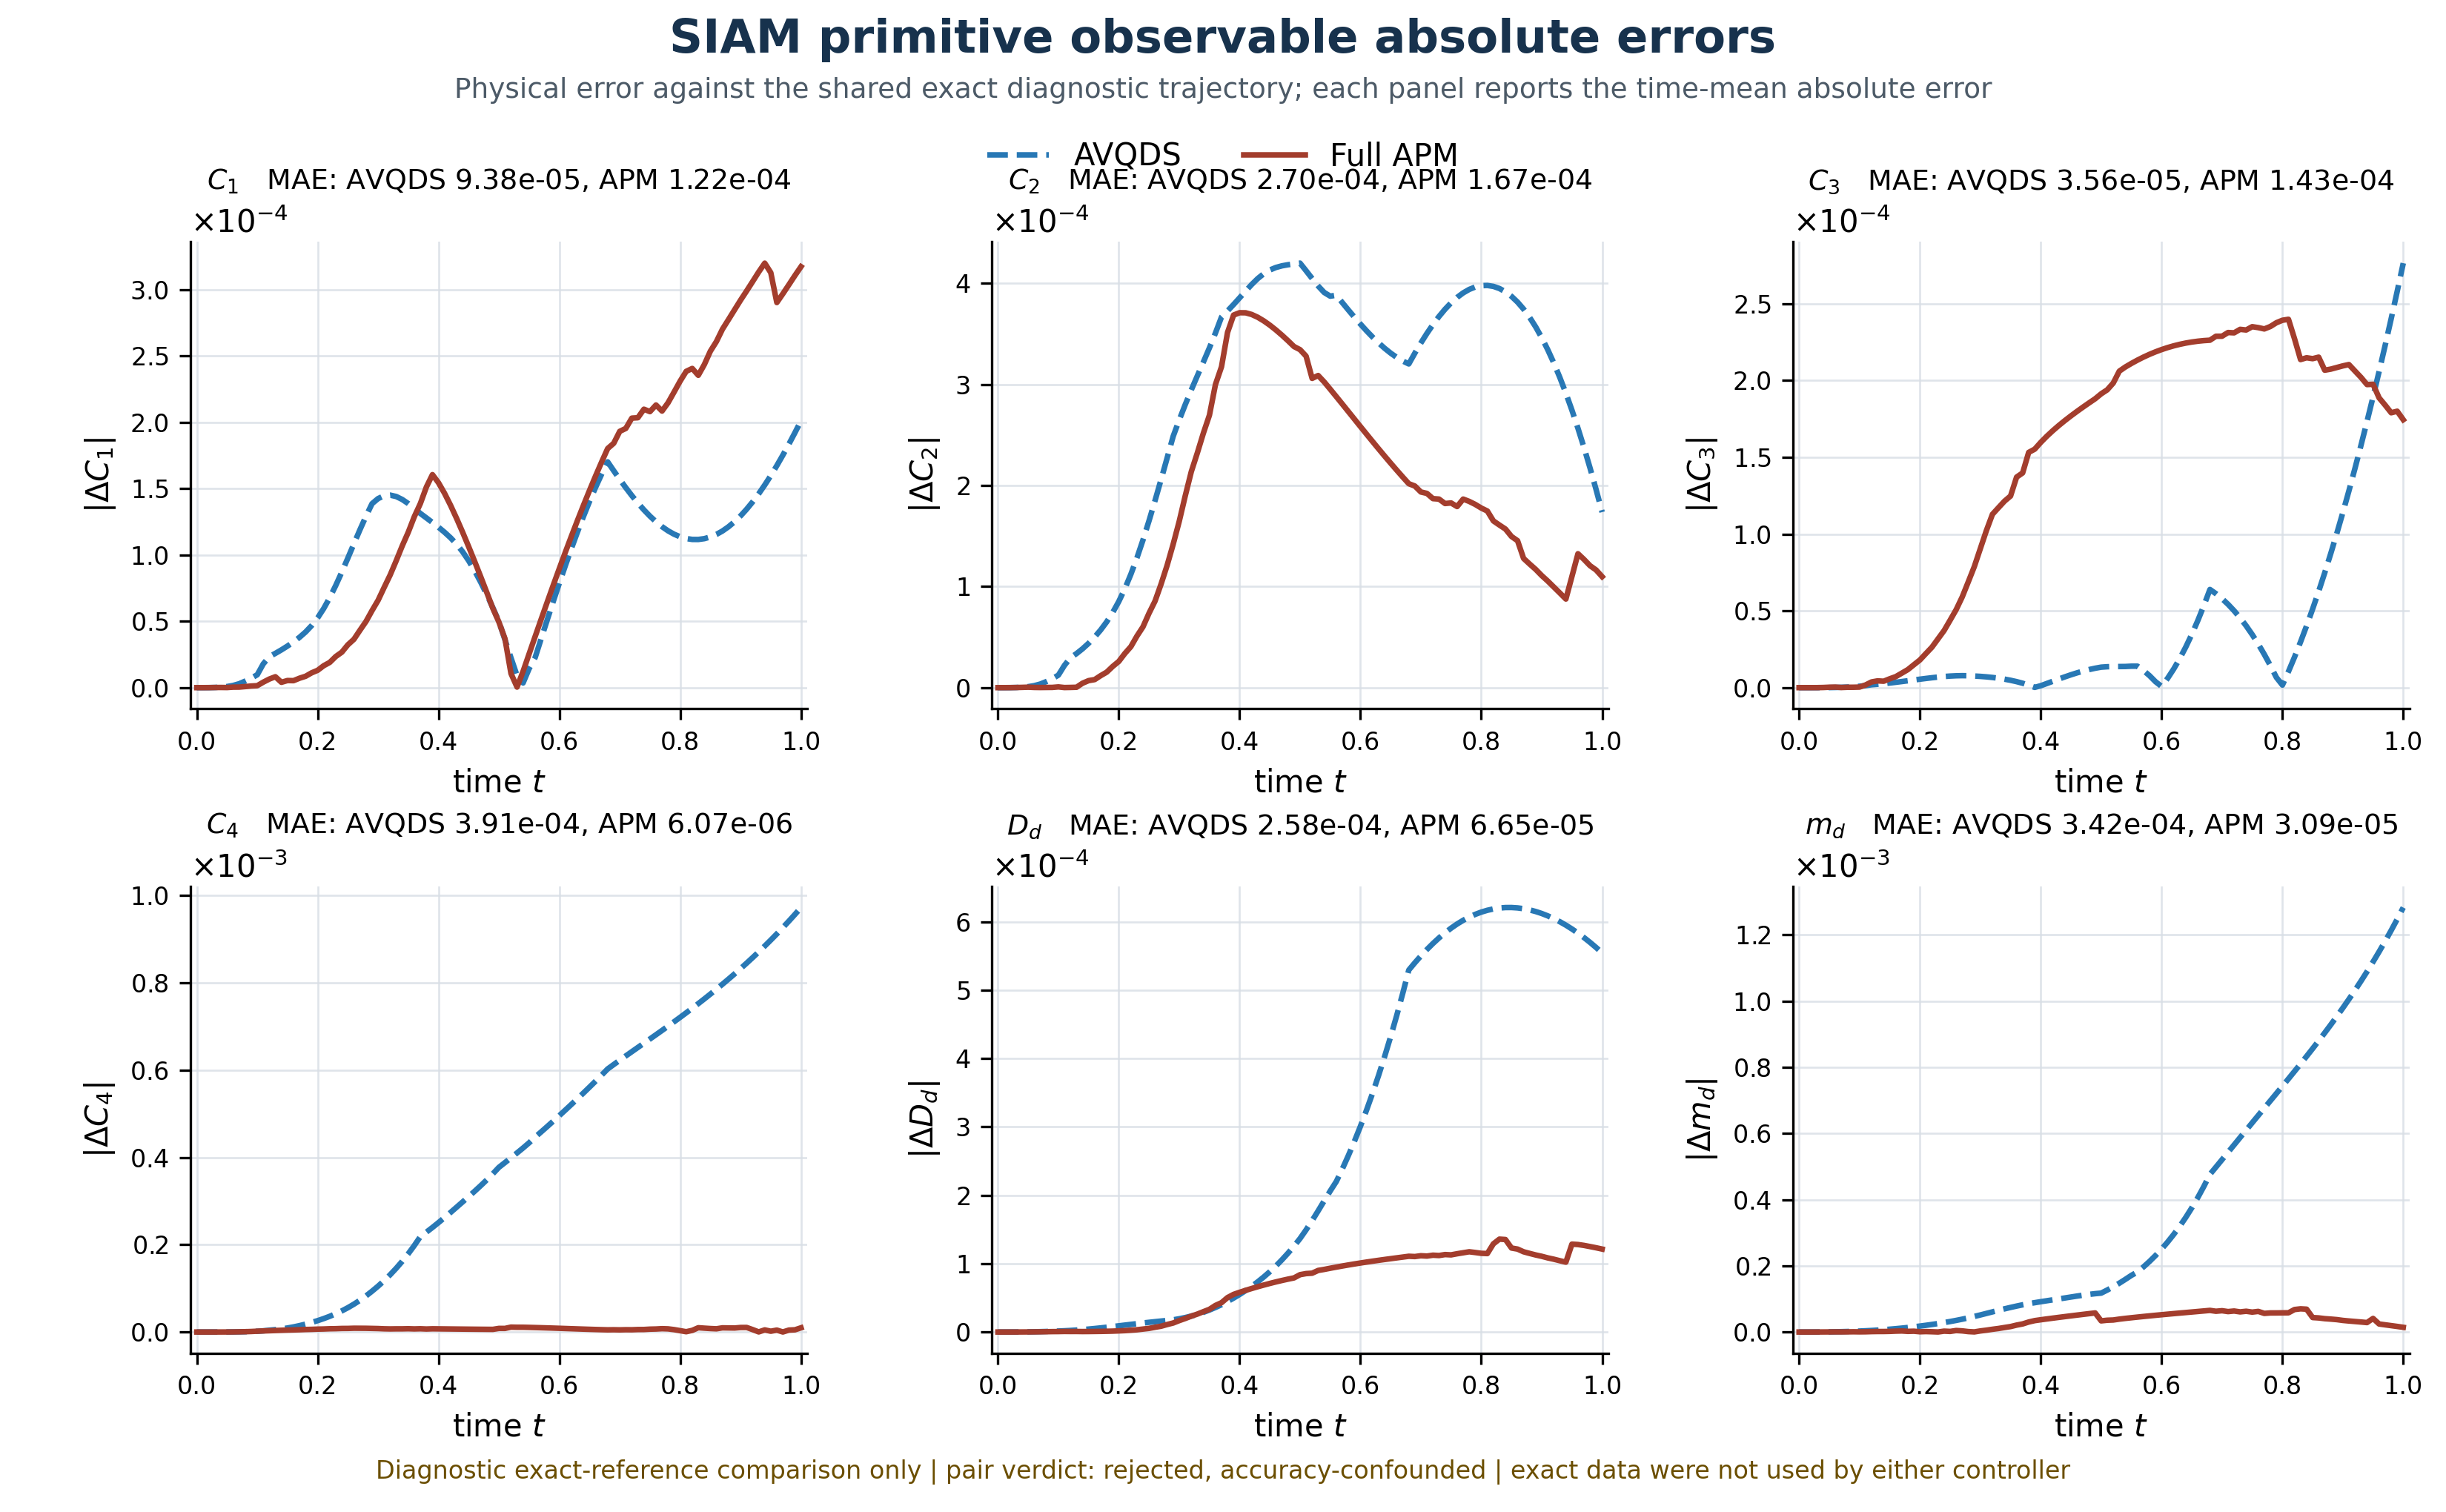
\includegraphics[width=\linewidth,height=7.15in,keepaspectratio]{siam_nb4_primitive_absolute_errors.png}
\end{center}

\newpage
\begin{center}
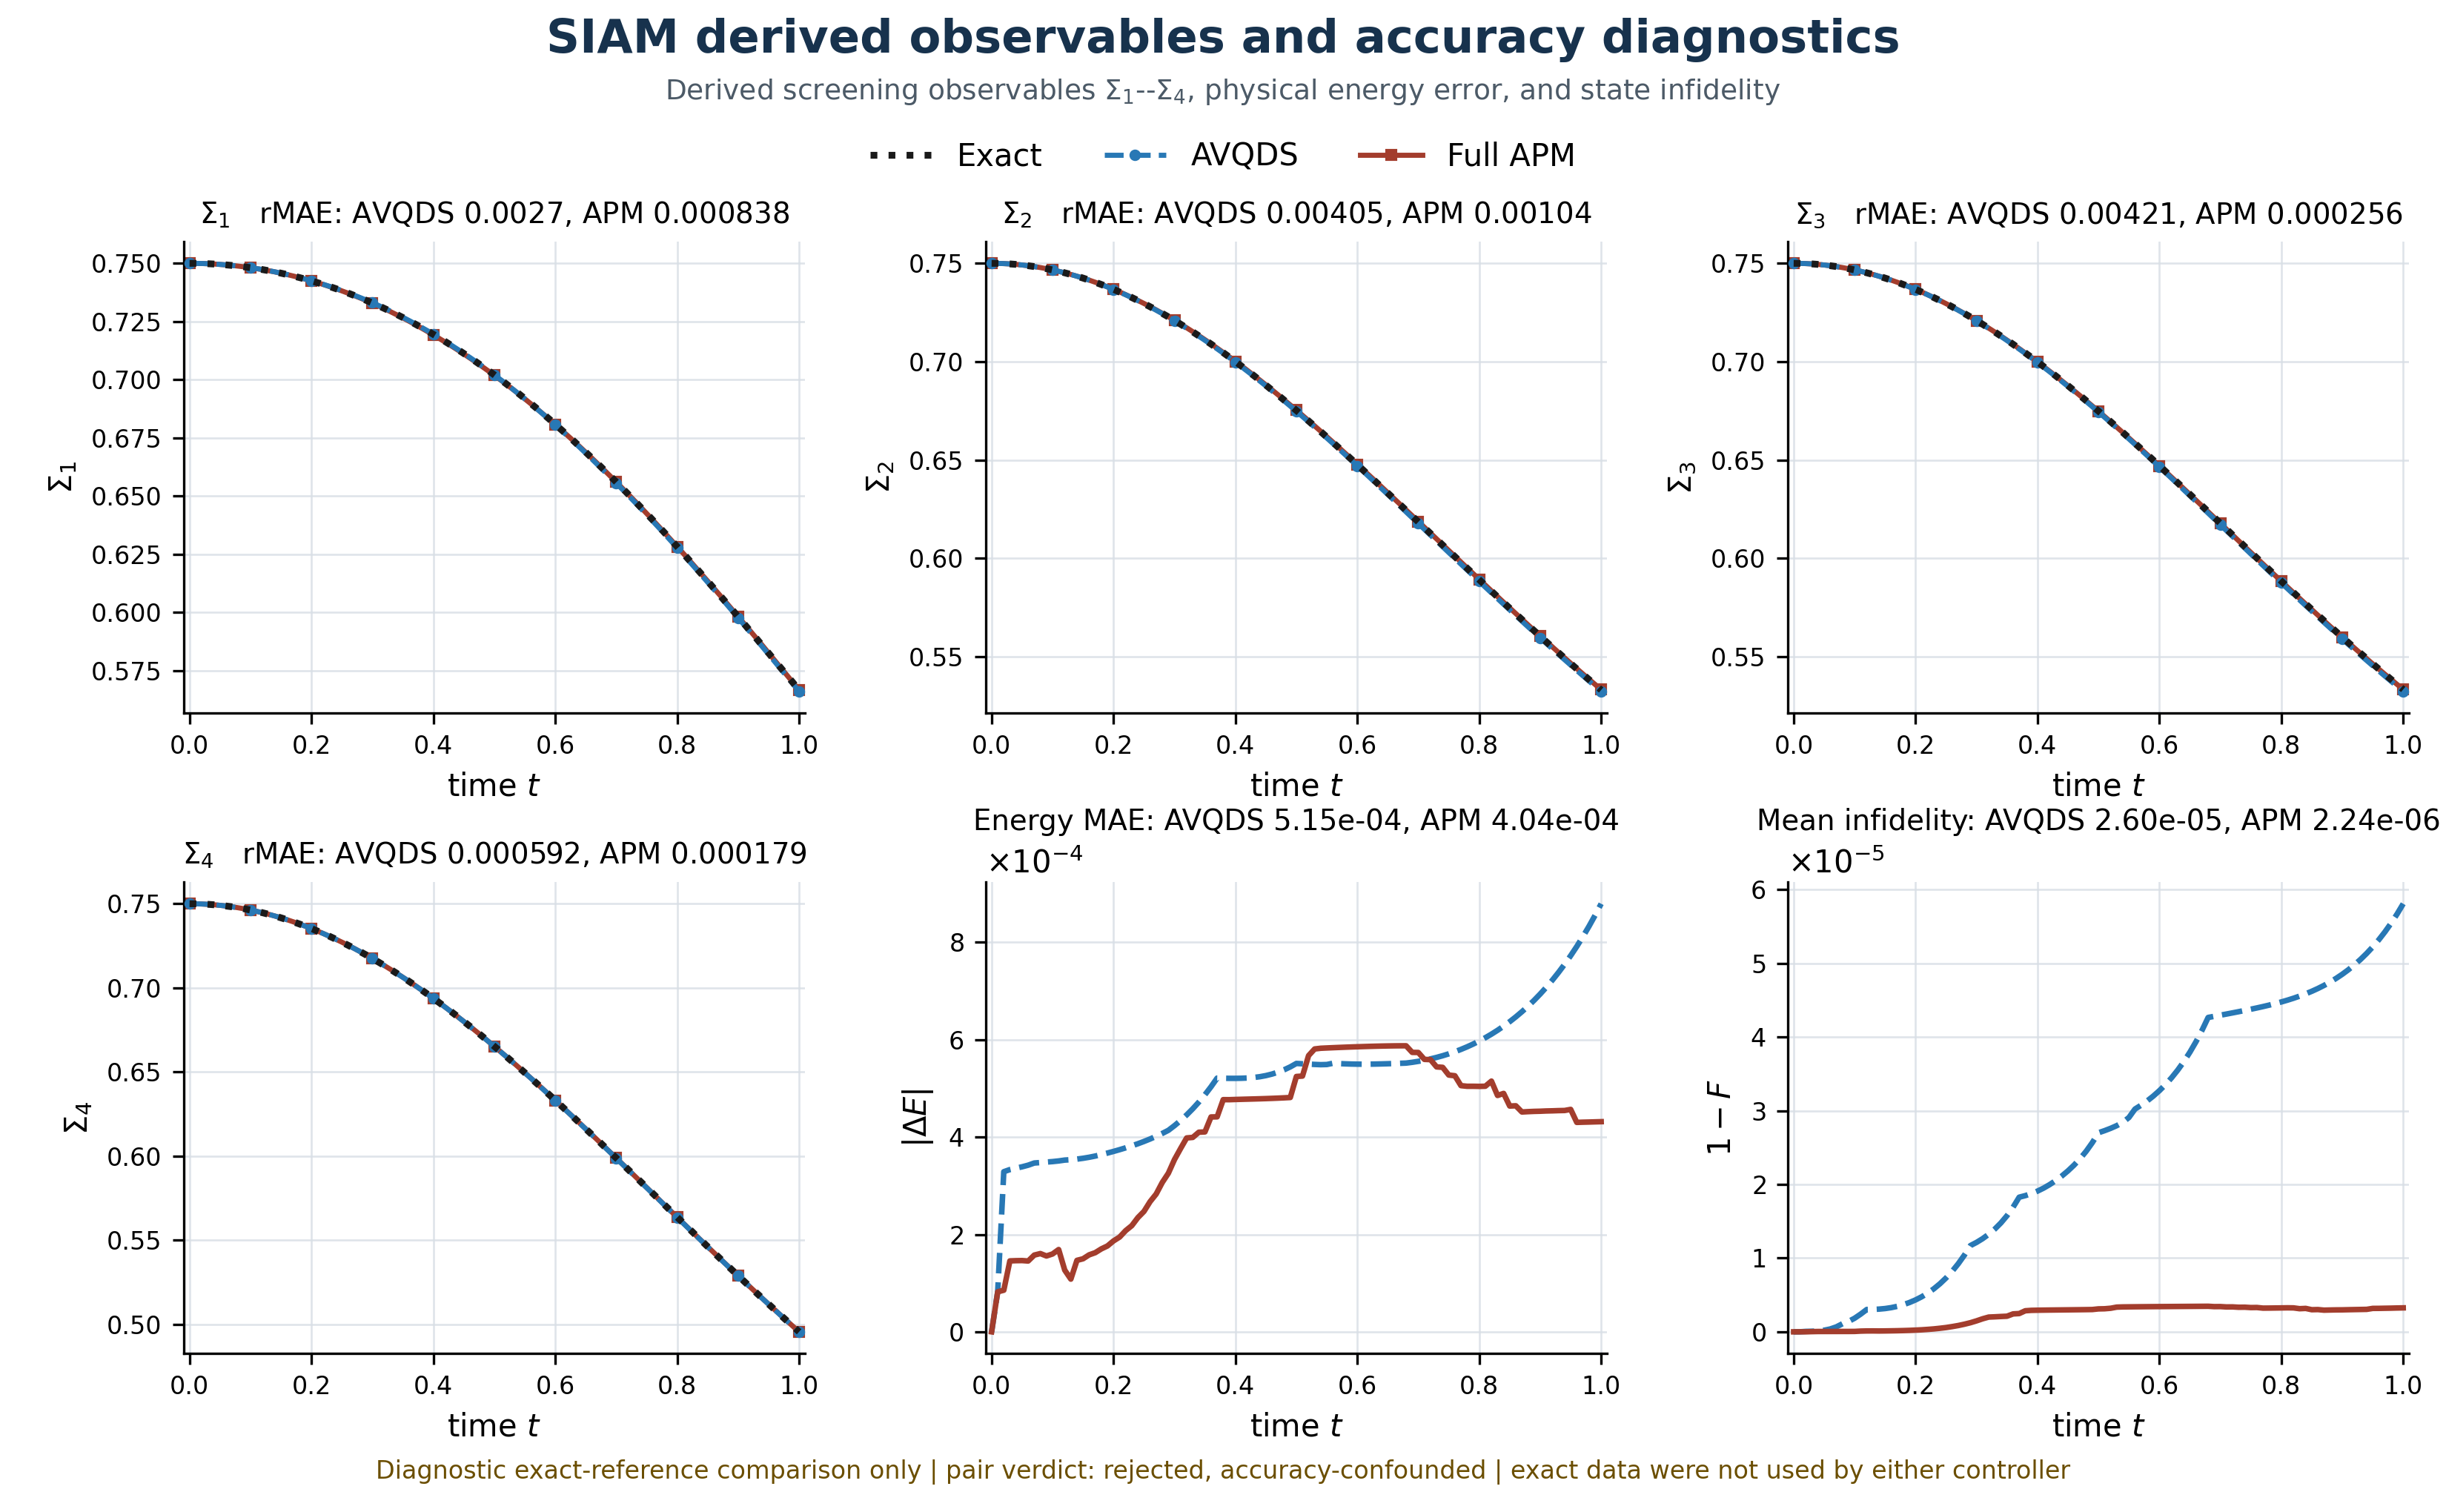
\includegraphics[width=\linewidth,height=7.15in,keepaspectratio]{siam_nb4_derived_and_accuracy.png}
\end{center}

\end{document}
